\documentclass{article}
\usepackage{graphicx}
\usepackage[margin=1in]{geometry}

% %
% \makeatletter
% \setlength{\@fptop}{0pt}
% \makeatother
% %

\begin{document}

\title{Supplementary material for ``Visualization methods for RNA-sequencing data analysis"}
\author{Lindsay Rutter}

\maketitle

\clearpage
\null
\begin{figure}[t!]
\centerline{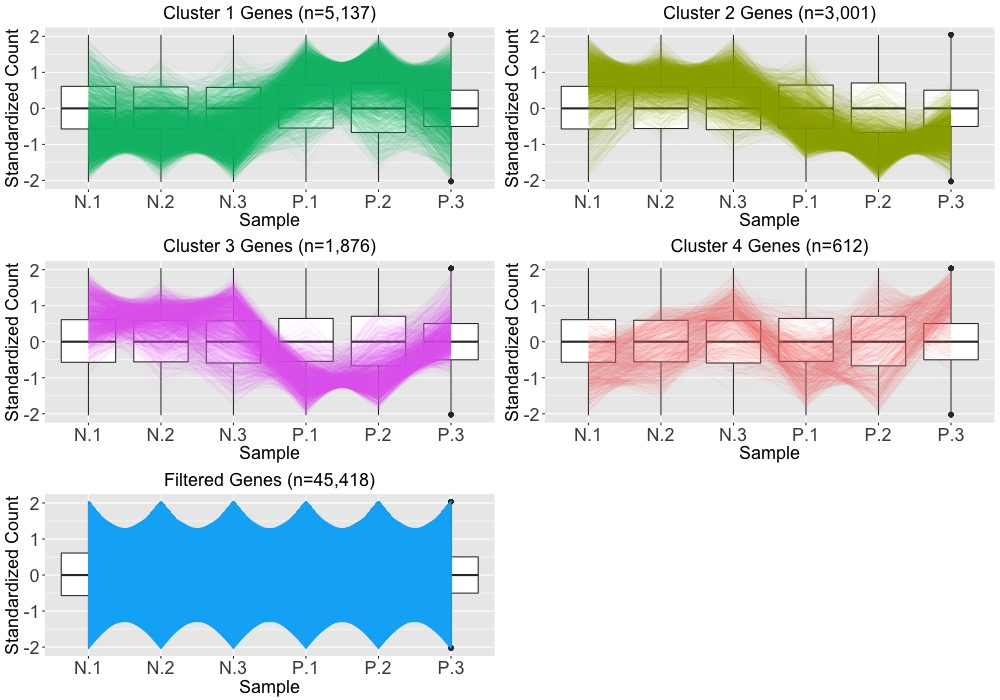
\includegraphics[width=\columnwidth]{../MakeFigures/sbIRClusters.jpg}}
\caption{Example application of parallel coordinate plots using the iron-metabolism soybean dataset. We filtered genes with low means and/or variance, performed a hierarchical clustering analysis with a cluster size of four, and visualized the results using parallel coordinate lines. Most non-filtered genes were in Clusters 1 and 2, which both showed overexpression in one treatment and underexpression in the other treatment. The genes in Cluster 4 mostly showed messy patterns with low signal to noise ratios. Interestingly, Cluster looked similar to Cluster 2 (large values for group N and small values for group P), except for unexpectedly large values for the third replicate of group P.
\label{sbIRClusters}}
\end{figure}

\clearpage
\null
\begin{figure}[t!]
\centerline{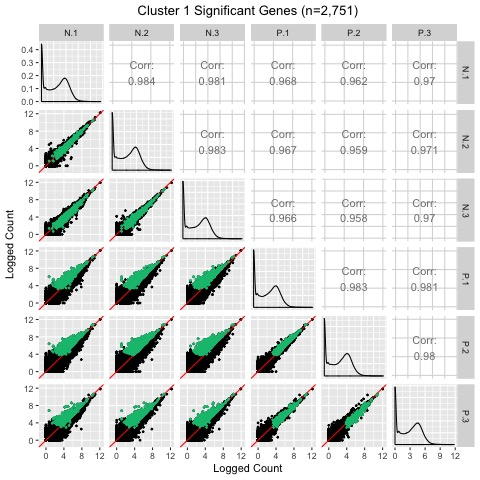
\includegraphics[width=\columnwidth]{../Bioinformatics/Pictures/FilterNotSig/Clustering_data_FDR_05/N_P_Sig_SM_4_1.jpg}}
\caption{Example of using a scatterplot matrix to assess DEG calls from a model in the iron-metabolism soybean dataset. There were 2751 significant genes in Cluster 1 after performing a hierarchical clustering analysis with a cluster size of four. These significant genes are overlaid in green over the scatterplot matrix. They follow the expected patterns of differential expression with most green points falling along the \textit{x=y} line in the scatterplots between replicates, but deviating from the \textit{x=y} line in the scatterplots between treatments. The deviation consistently demonstrates higher expression in the P group than in the N group. Hence, these green points seem to represent genes that were significantly overexpressed in the P group, which draws the same conclusion with what we derived using the parallel coordinate plots in Figure 2 of the paper. One difficulty with plotting such a large number of DEGs onto the scatterplot matrix is that overplotting can obscure our inability to determine how many DEGs are in a given location.
\label{suppSMCluster1}}
\end{figure}

\clearpage
\null
\begin{figure}[t!]
\centerline{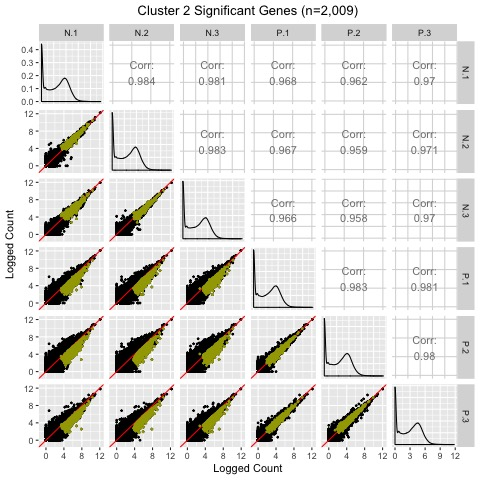
\includegraphics[width=\columnwidth]{../Bioinformatics/Pictures/FilterNotSig/Clustering_data_FDR_05/N_P_Sig_SM_4_2.jpg}}
\caption{Example of using a scatterplot matrix to assess DEG calls from a model in the iron-metabolism soybean dataset. There were 2009 significant genes in Cluster 2 after performing a hierarchical clustering analysis with a cluster size of four. These significant genes are overlaid in mustard over the scatterplot matrix. They follow the expected patterns of differential expression with most mustard points falling along the \textit{x=y} line in the scatterplots between replicates, but deviating from the \textit{x=y} line in the scatterplots between treatments. The deviation consistently demonstrates higher expression in the N group than in the P group. Hence, these mustard points seem to represent genes that were significantly overexpressed in the N group, which draws the same conclusion with what we derived using the parallel coordinate plots in Figure 2 of the paper. One difficulty with plotting such a large number of DEGs onto the scatterplot matrix is that overplotting can obscure our inability to determine how many DEGs are in a given location.
\label{suppSMCluster2}}
\end{figure}
  
\null
\begin{figure}[t!]
\centerline{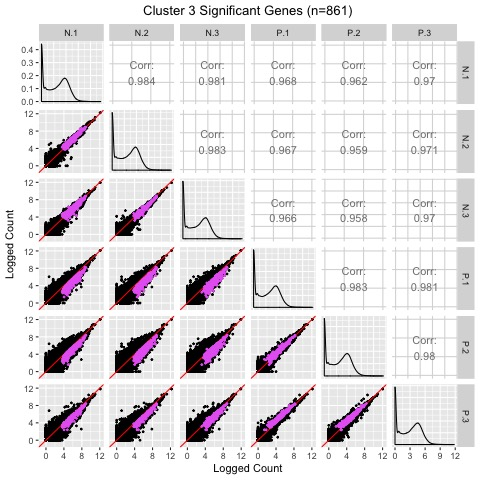
\includegraphics[width=\columnwidth]{../Bioinformatics/Pictures/FilterNotSig/Clustering_data_FDR_05/N_P_Sig_SM_4_3.jpg}}
\caption{Example of using a scatterplot matrix to assess DEG calls from a model in the iron-metabolism soybean dataset. There were 861 significant genes in Cluster 3 after performing a hierarchical clustering analysis with a cluster size of four. These significant genes are overlaid in pink over the scatterplot matrix. For the most part, they follow the expected patterns of differential expression with pink points falling along the \textit{x=y} line in the scatterplots between replicates, but deviating from the \textit{x=y} line in the scatterplots between treatments. The deviation consistently demonstrates higher expression in the N group than in the P group. However, the scatterplot between replicates P.1 and P.3 show slightly higher expression in P.3, and the scatterplot between replicates P.2 and P.3 also show slightly higher expression in P.3. Hence, these pink points seem to represent genes that were significantly overexpressed in the N group, but with slight inconstencies in the replicates in the P group. The parallel coordinate plots in Figure 2 of the paper showed this same conclusion and perhaps more clearly. One difficulty with plotting such a large number of DEGs onto the scatterplot matrix is that overplotting can obscure our inability to determine how many DEGs are in a given location.
\label{suppSMCluster3}}
\end{figure}  

\clearpage
\null
\begin{figure}[t!]
\centerline{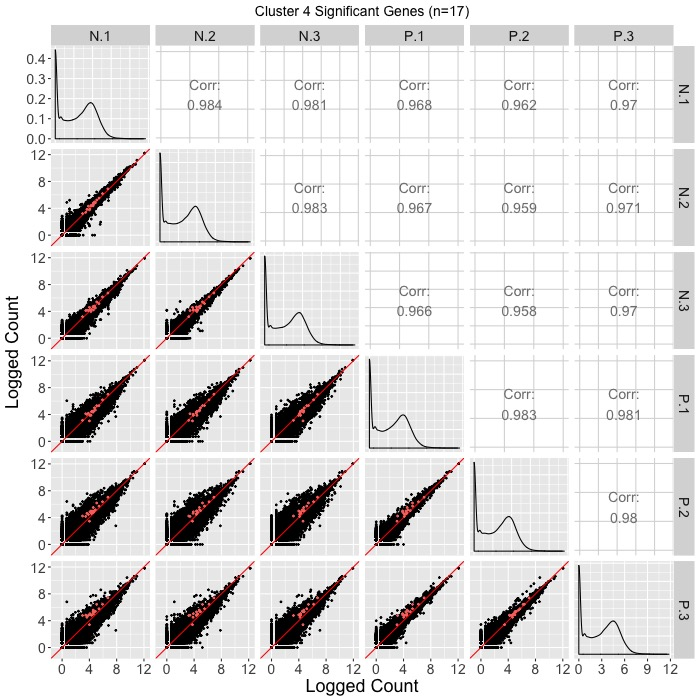
\includegraphics[width=\columnwidth]{../Bioinformatics/Pictures/FilterNotSig/Clustering_data_FDR_05/N_P_Sig_SM_4_4.jpg}}
\caption{Example of using a scatterplot matrix to assess DEG calls from a model in the iron-metabolism soybean dataset. There were 17 significant genes in Cluster 4 after performing a hierarchical clustering analysis with a cluster size of four. These significant genes are overlaid in coral over the scatterplot matrix. For the most part, they do not seem to follow the expected patterns of differential expression: In many of the scatterplots between treatments, the coral points do not seem to deviate much from the \textit{x=y} line. Moreover, in the scatterplots between P.1 and P.2 as well as P.1 and P.3, the coral points seems to indicate an underexpression of the P.1 replicate. We found a similar finding of somewhat messy looking DEG calls in Cluster 4 from Figure 2 in the paper. 
\label{suppSMCluster4}}
\end{figure}  
 
\clearpage
\null 
\begin{figure}[t!]
\centerline{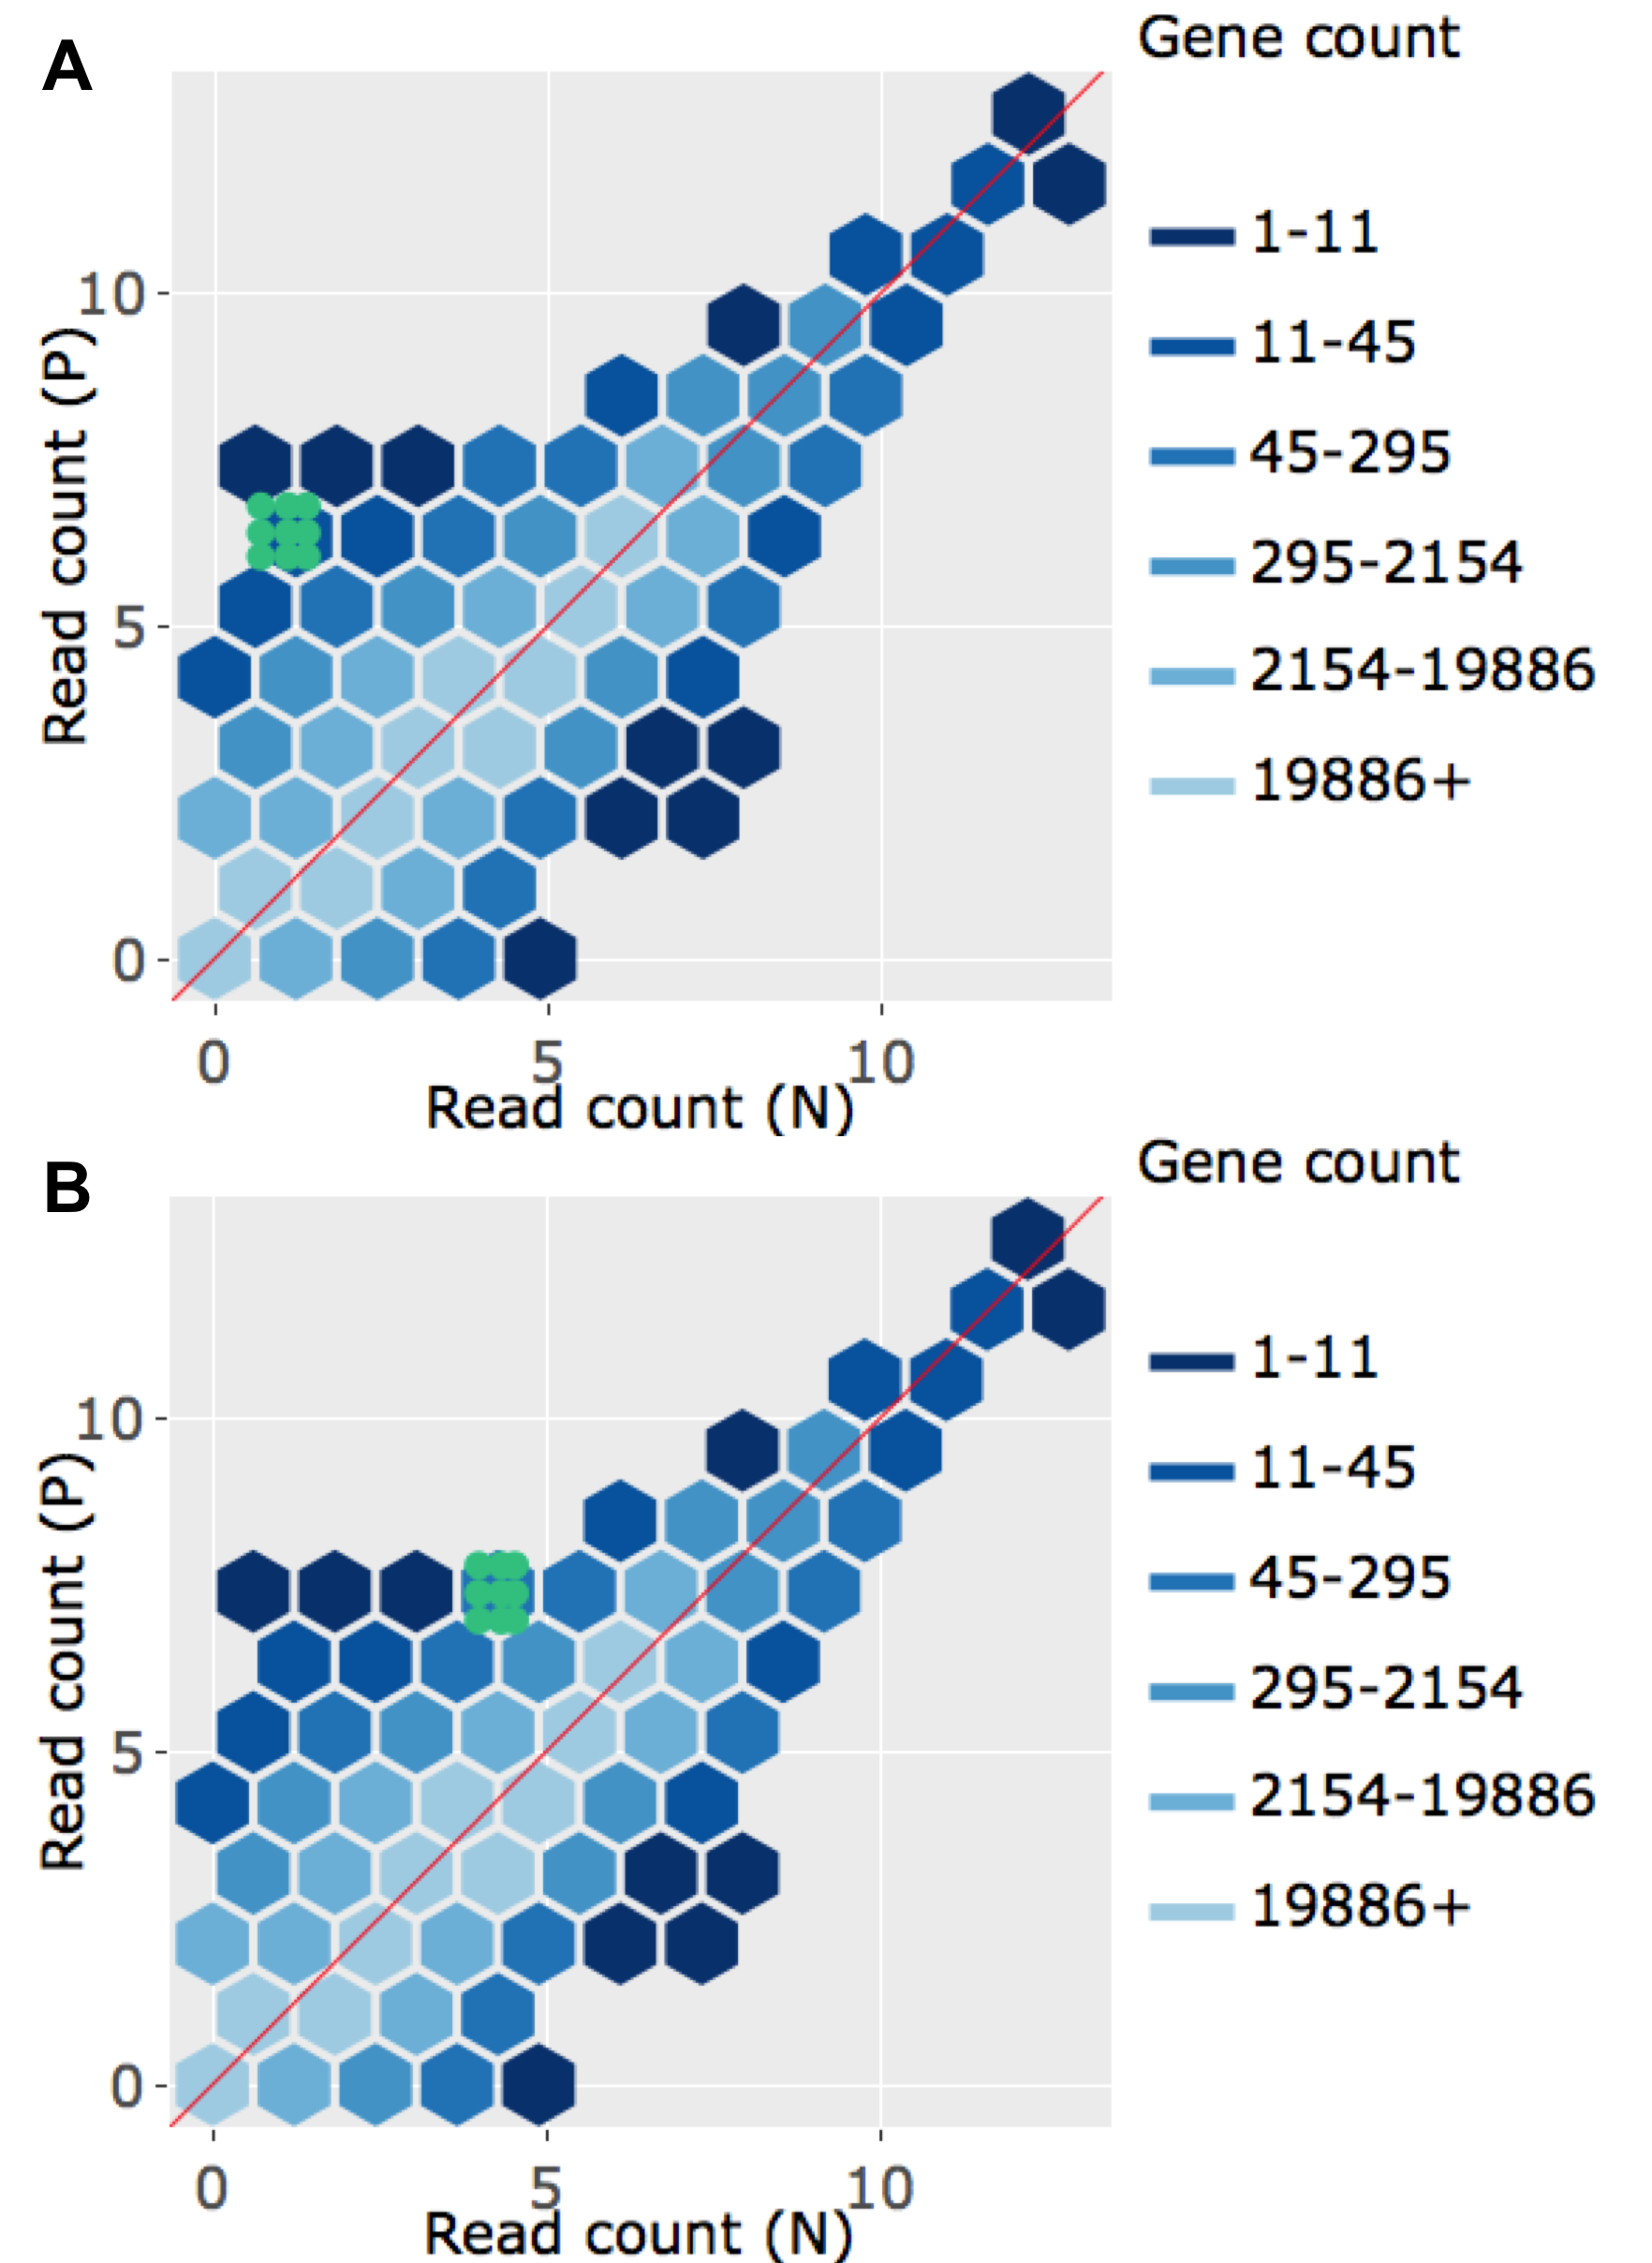
\includegraphics[width=0.7\columnwidth]{../Bioinformatics/Pictures/litrePlots/N_P/litreCluster1.png}}
\caption{Litre plots for significant genes inside Cluster 1 from Figure 2 of the paper. Subplots A and B each overlay a significant gene from Cluster 1 as nine green points. The genes show a pattern expected of a differentially-expressed one, by clumping together and deviating from the \textit{x=y} line. Moreover, the genes appear over-expressed in the P group. This is consistent with what we saw in Figure 2 of the paper. To interactively view the litre plot for all significant genes within Cluster 1, please visit https://rnaseqvisualization.shinyapps.io/litreCluster1.
\label{litreCluster1}}
\end{figure}   

%%%%%%%%%%%%%%%%%%%% Check percent signs in captions! %%%%%%%%%%%%%%%%%%%% 

\clearpage
\null
\begin{figure}[t!]
\centerline{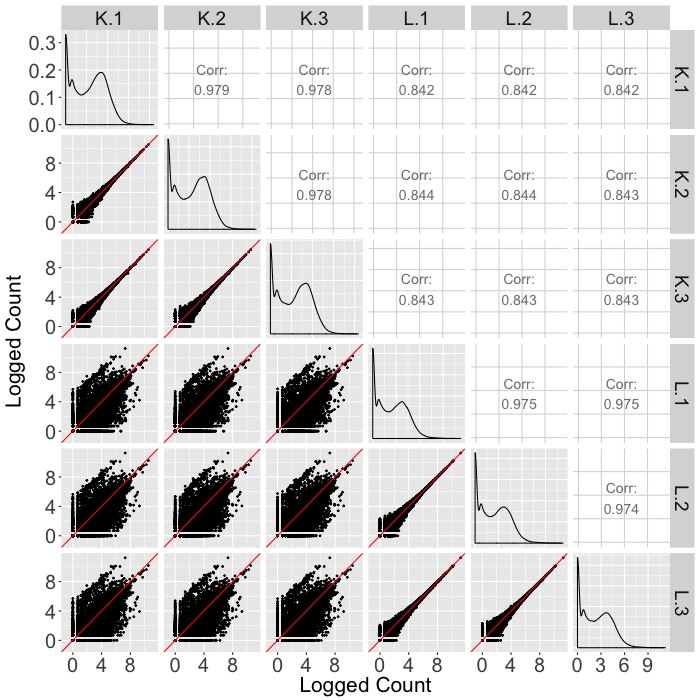
\includegraphics[width=1\columnwidth]{../Bioinformatics/Pictures/liverKidney/DEG-raw/K_L_SM.jpg}}
\caption{Scatterplot matrix of liver and kidney technical replicates. The technical replicate scatterplots look as precise as expected, with little variability around the \textit{x=y} line. The treatment group scatterplots have much more variability around the \textit{x=y} line, as we would expect. However, each treatment group scatterplot contains a pronounced streak of highly-expressed liver-specific genes, which deviates from the expected distribution. Some researchers have suggested that differences in the distribution of reads between groups may require more stringent normalization than library scaling, such as TMM normalization.
\label{KLSM}}
\end{figure}

\clearpage
\null
\begin{figure}[t!]
\centerline{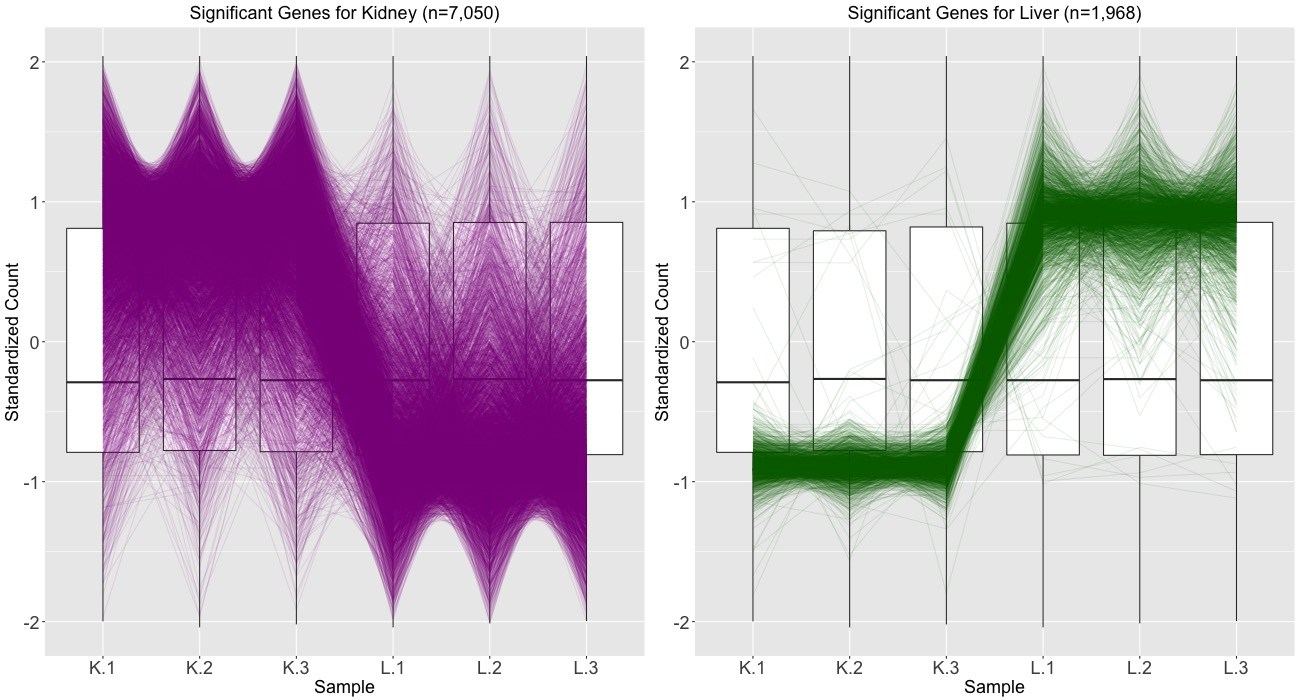
\includegraphics[width=1\columnwidth]{../Bioinformatics/Pictures/liverKidney/Clustering_data_FDR_001_Raw/Alpha0.1/K_L_Sig.jpg}}
\caption{Parallel coordinate plots of the DEGs from liver and kidney technical replicates after standard library scale normalization. The division of DEGs between the two groups was rather disparate, with ~78\% of the DEGs being kidney-specific and only ~22\% of the DEGs being liver-specific. Also of note, while the parallel coordinate patterns of the liver-specific DEGs appear as expected, the patterns of the kidney-specific DEGs seem to show comparatively much larger variability between the replicates.
\label{RawKLSig}}
\end{figure}   

\clearpage
\null
\begin{figure}[t!]
\centerline{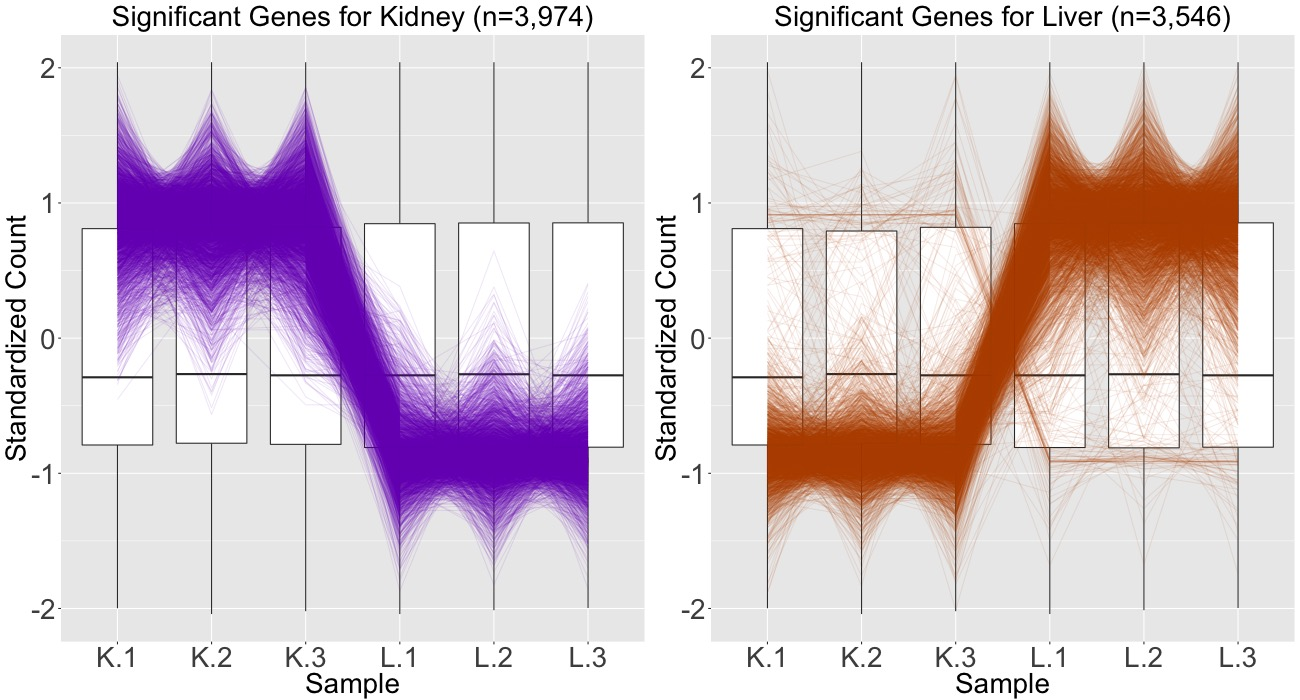
\includegraphics[width=1\columnwidth]{../Bioinformatics/Pictures/liverKidney/Clustering_data_FDR_001_TMM/Alpha0.1/K_L_Sig.jpg}}
\caption{Parallel coordinate plots of the DEGs from liver and kidney technical replicates after TMM normalization. The division of DEGs between the two groups is more balanced than in Figure~\ref{RawKLSig}, with ~53\% of the DEGs being kidney-specific and ~47\% of the DEGs being liver-specific. Additionally, the parallel coordinate patterns of both the liver-specific and kidney-specific DEGs appear as expected and more consistent with each other.
\label{TMMKLSig}}
\end{figure} 

\null
\begin{figure}[t!]
\centerline{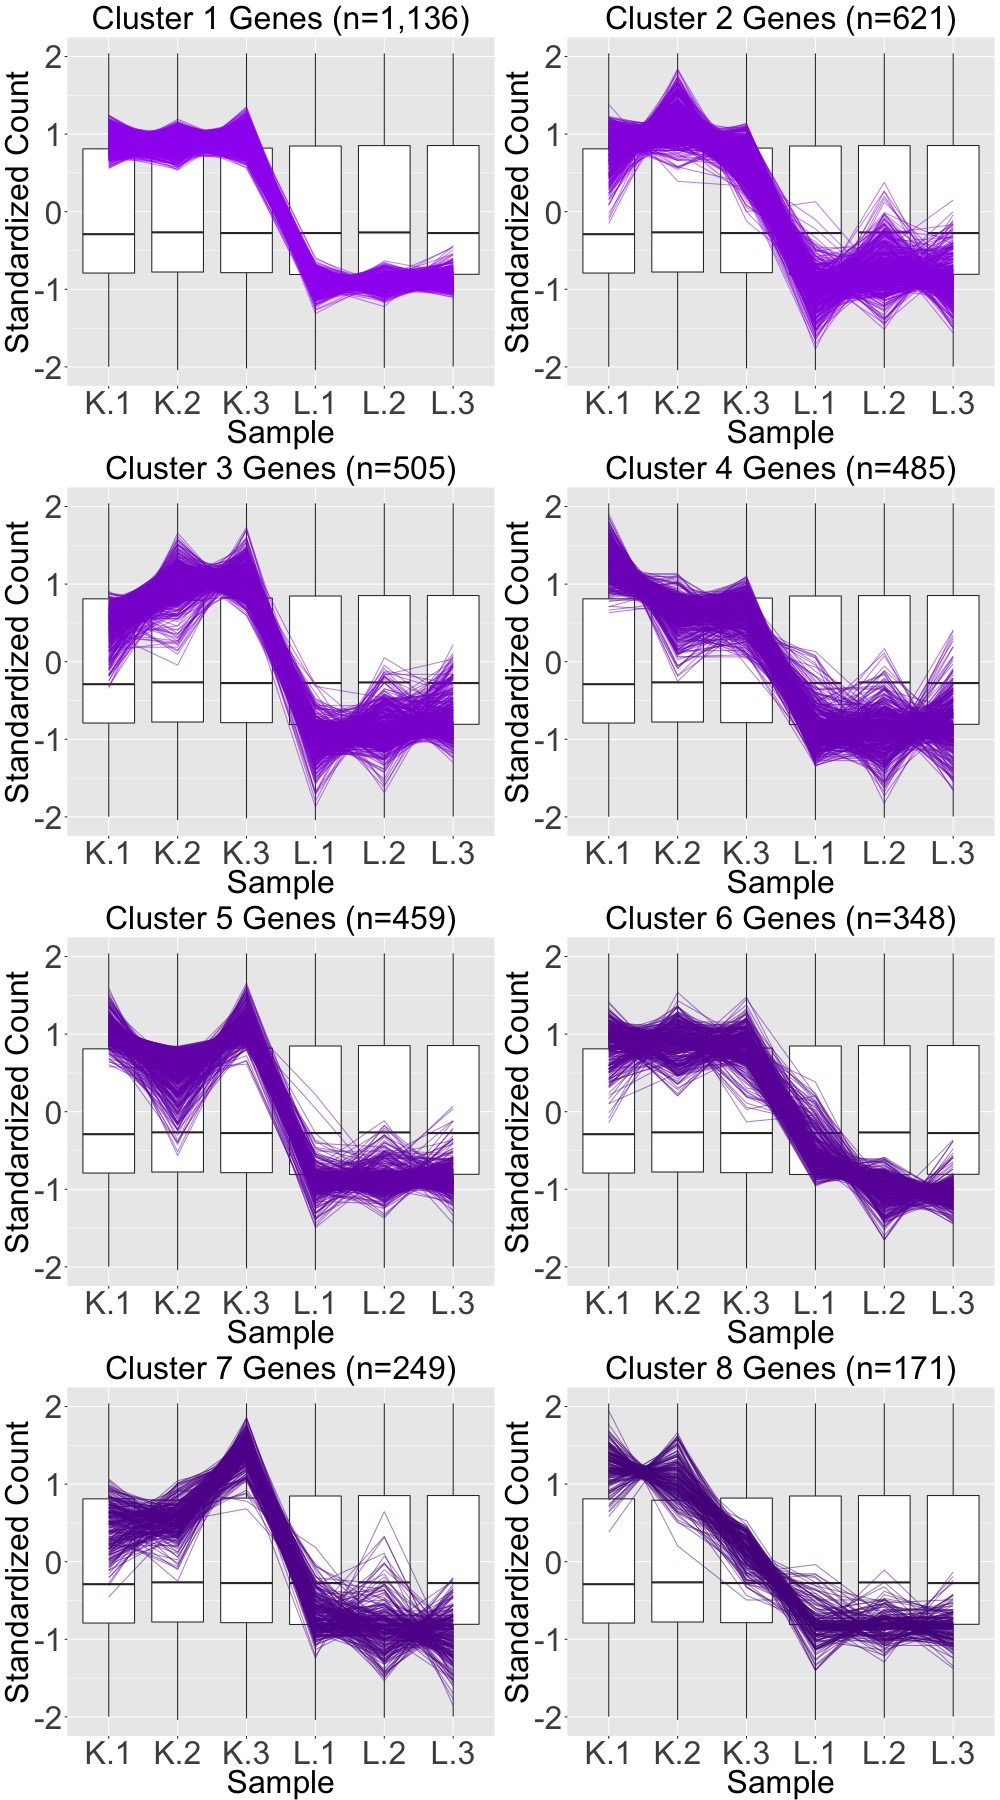
\includegraphics[width=0.65\columnwidth]{../Bioinformatics/Pictures/liverKidney/Clustering_data_FDR_001_TMMvRaw_Keep/K_L_8.jpg}}
\caption{Parallel coordinate plots showing hiearchical clustering analysis results of size eight for the 3,974 genes that remained in the kidney-specific DEGs after TMM normalization. We see that, for the most part, the parallel coordinate patterns follow the expected patterns across the clusters. The ideal pattern of DEGs is especially captured in the first cluster (the largest one with 1,136 genes). We used hierarchical clustering to mitigate additional overplotting that would occur if we were to plot all genes onto only one parallel coordinate plot.
\label{KeepPCP}}
\end{figure}

\null
\begin{figure}[t!]
\centerline{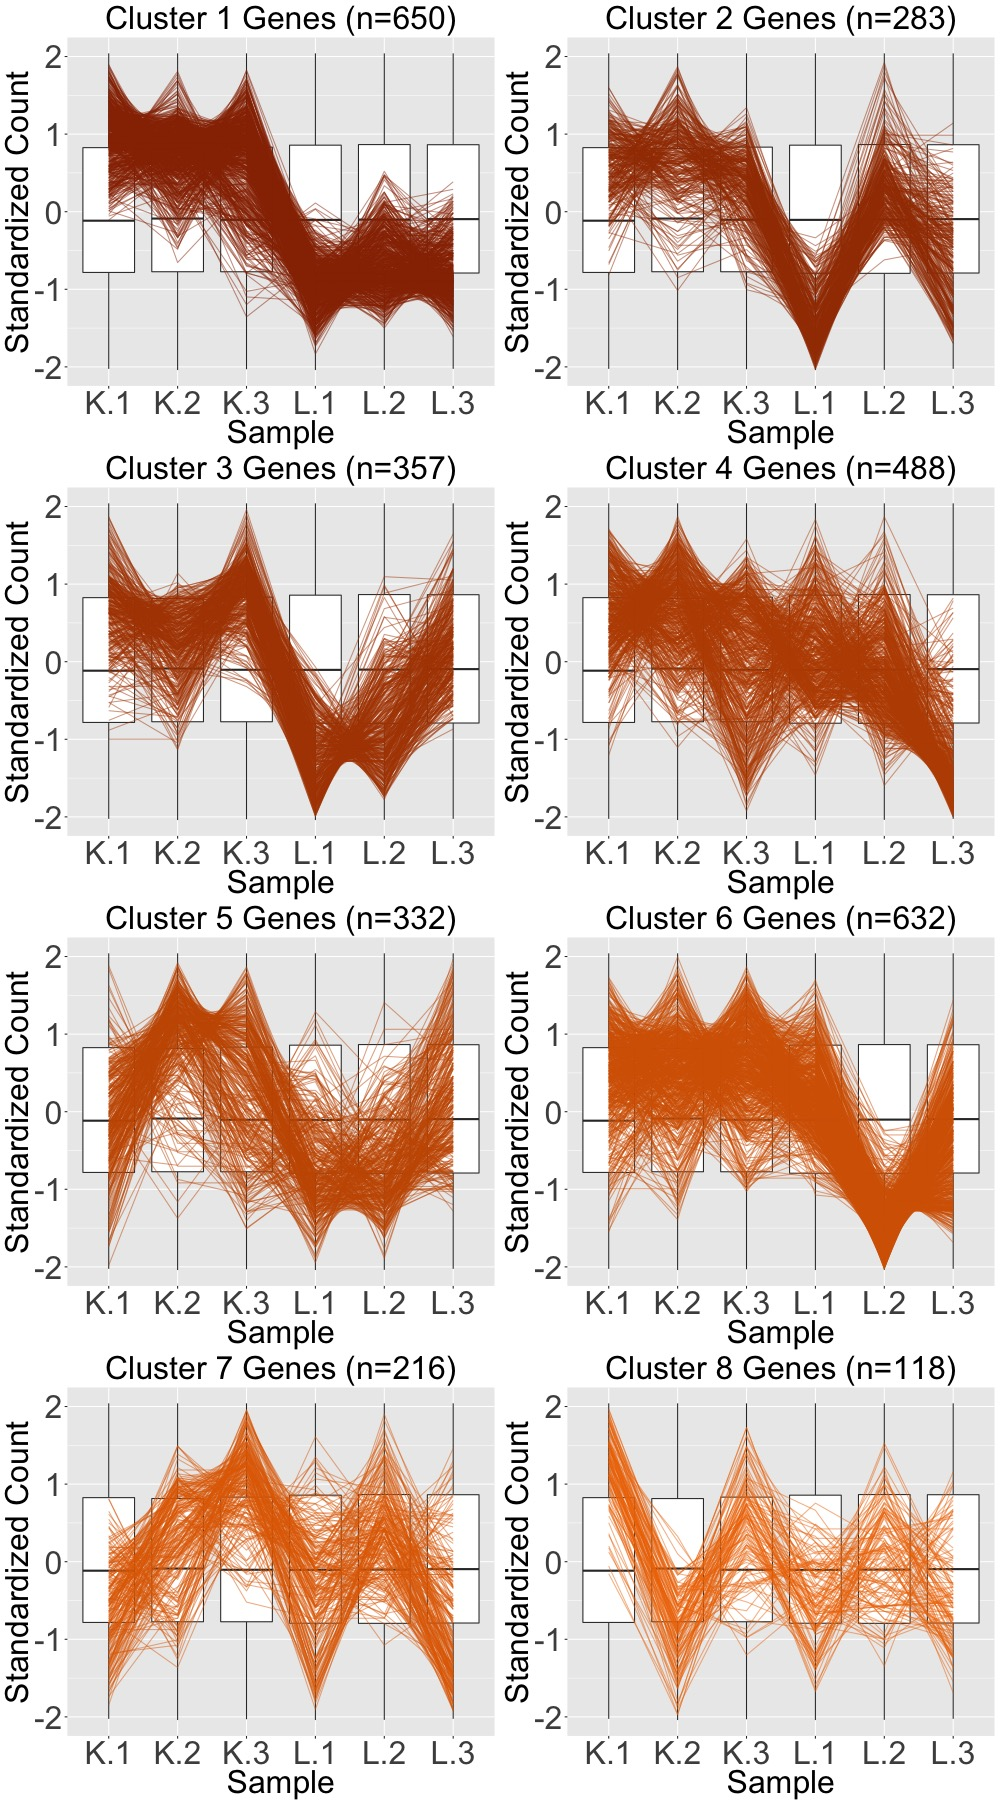
\includegraphics[width=0.65\columnwidth]{../Bioinformatics/Pictures/liverKidney/Clustering_data_FDR_001_TMMvRaw_Removed/K_L_8.jpg}}
\caption{Parallel coordinate plots showing hiearchical clustering analysis results of size eight for the 3,076 genes that were removed from the kidney-specific DEGs after TMM normalization. Unlike in Figure~\ref{KeepPCP}, the patterns in almost all clusters do not resemble the expected DEG format; instead, they show large variability between replicates and small variability between groups. In some clusters, it is difficult to even determine which group would be the overexpressed one if its genes were in fact DEGs. Taken together, this plot provides additional statistical evidence that the application of TMM normalization successfully removed genes that were previously mislabeled as kidney-specific DEGs (in Figure~\ref{RawKLSig}) with library scaling normalization. We used hierarchical clustering to mitigate additional overplotting that would occur if we were to plot all genes onto only one parallel coordinate plot.
\label{RemovePCP}}
\end{figure}

\null
\begin{figure}[t!]
\centerline{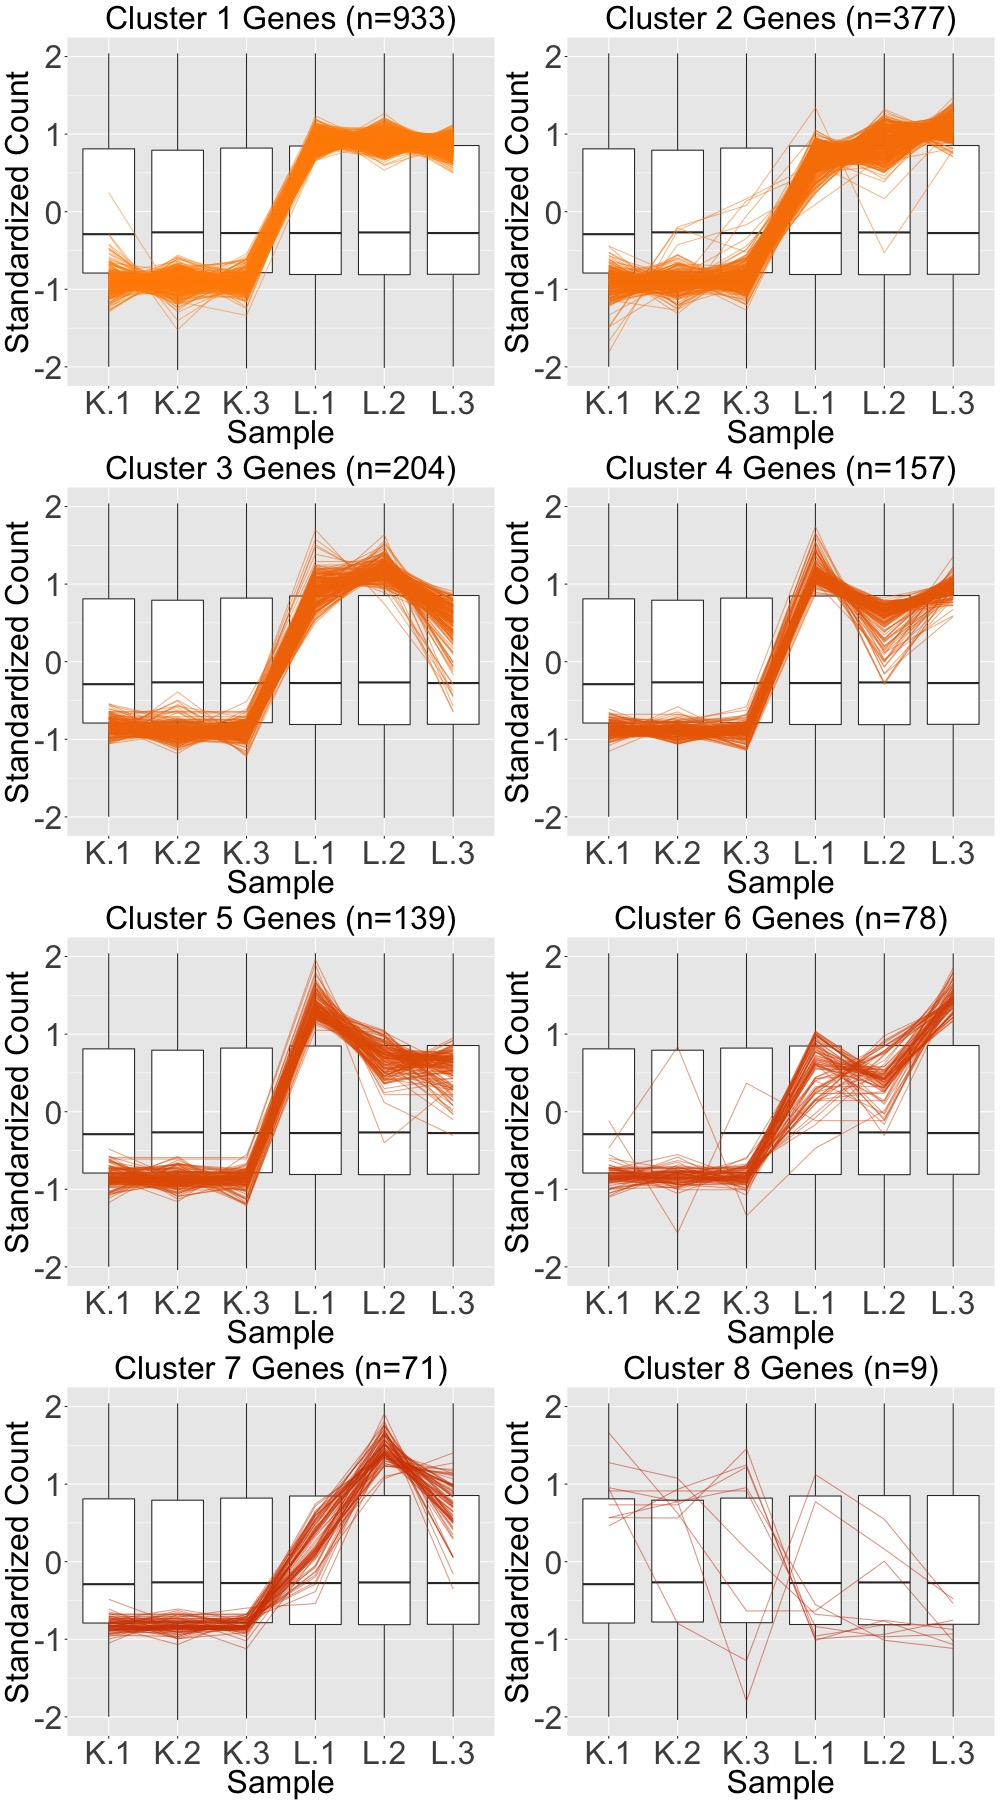
\includegraphics[width=0.65\columnwidth]{../Bioinformatics/Pictures/liverKidney/Clustering_data_FDR_001_TMMvRaw_Orig/K_L_8.jpg}}
\caption{Parallel coordinate plots showing hiearchical clustering analysis results of size eight for the 1,968 genes that were initially designated liver-specific DEGs after library scale normalization. We see that, for the most part, the parallel coordinate patterns follow the expected patterns across the clusters. The ideal pattern of DEGs is especially captured in the first cluster (the largest one with 933 genes). We used hierarchical clustering to mitigate additional overplotting that would occur if we were to plot all genes onto only one parallel coordinate plot.
\label{OrigPCP}}
\end{figure}

\null
\begin{figure}[t!]
\centerline{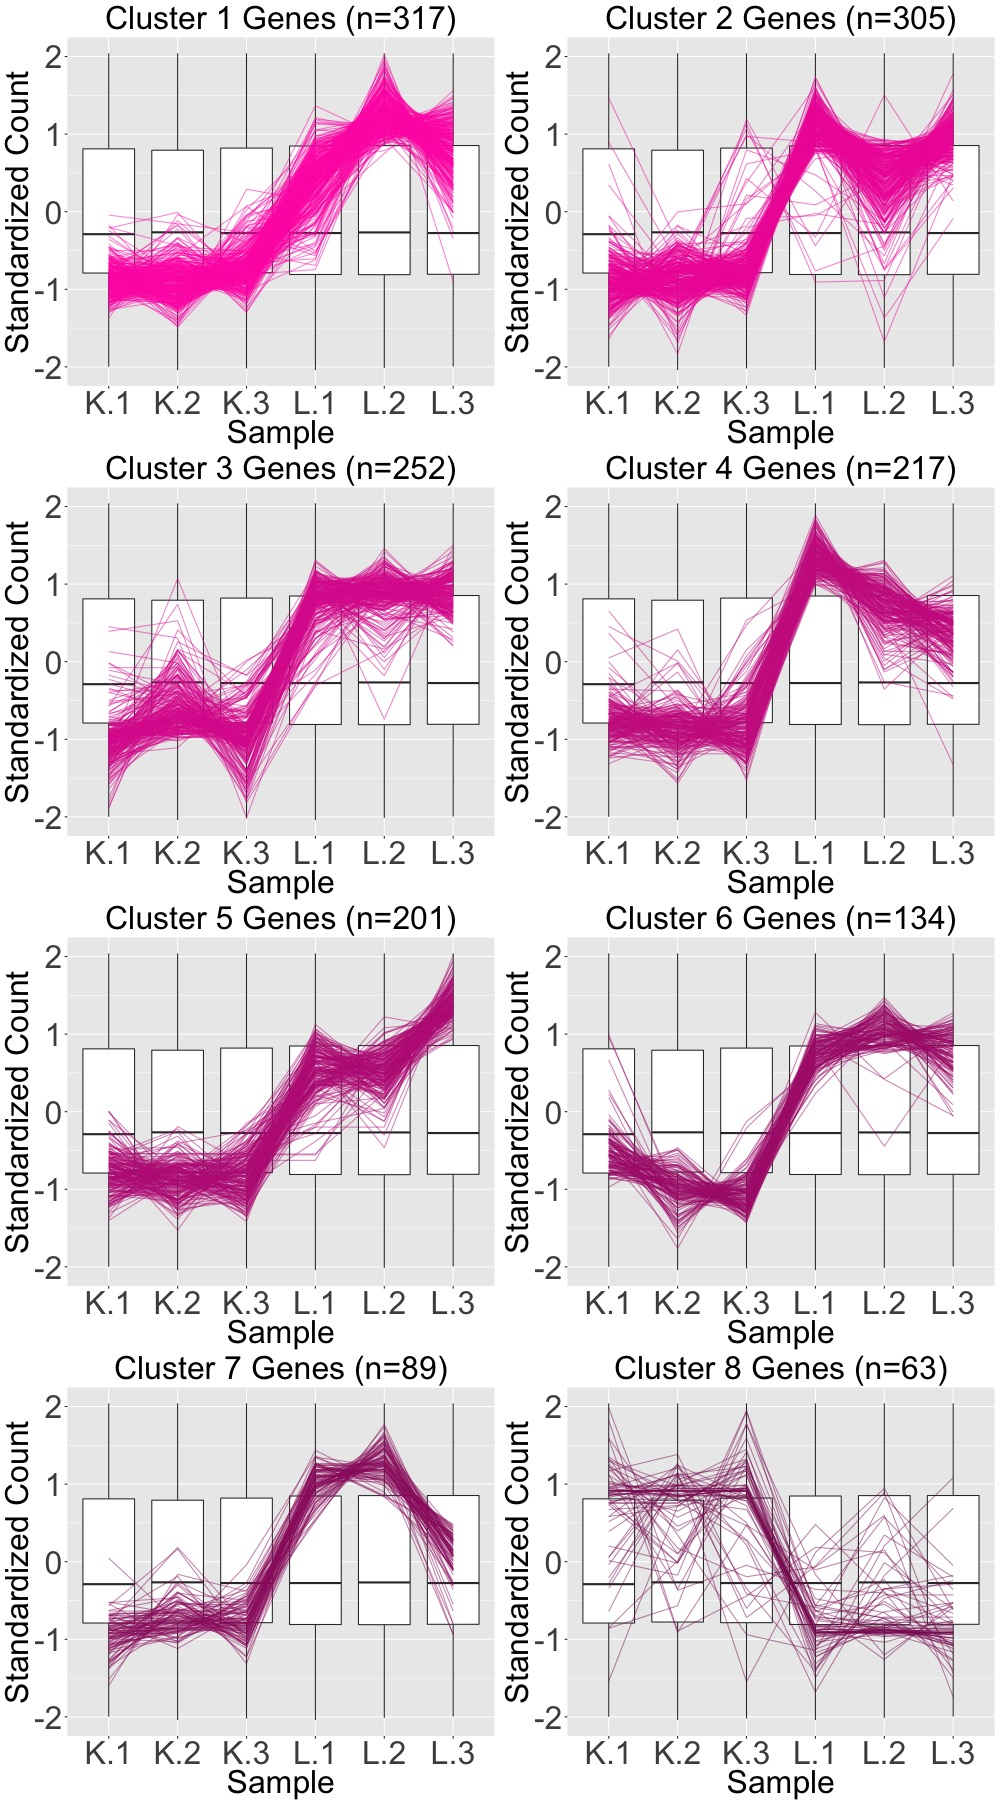
\includegraphics[width=0.65\columnwidth]{../Bioinformatics/Pictures/liverKidney/Clustering_data_FDR_001_TMMvRaw_Add/K_L_8.jpg}}
\caption{Parallel coordinate plots showing hiearchical clustering analysis results of size eight for the 1,578 genes that were \textit{added} as liver-specific DEGs after TMM normalization. We see that, for the most part, the parallel coordinate patterns follow the expected patterns across the clusters. We used hierarchical clustering to mitigate additional overplotting that would occur if we were to plot all genes onto only one parallel coordinate plot.
\label{AddPCP}}
\end{figure}

\null
\begin{figure}[t!]
\centerline{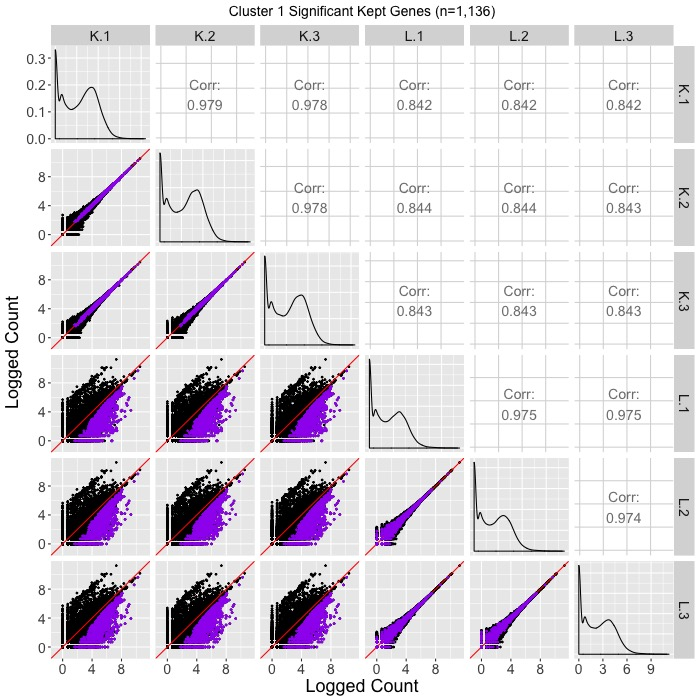
\includegraphics[width=1\columnwidth]{../Bioinformatics/Pictures/liverKidney/Clustering_data_FDR_001_TMMvRaw_Keep/K_L_Sig_SM_Keep_8_1.jpg}}
\caption{Scatterplot matrix of the 1,136 genes that were in the first cluster (of Figure~\ref{KeepPCP}) from genes that remained as kidney-specific DEGs even after TMM normalization. With this scatterplot matrix, we verify from an additional perspective that these genes demonstrate the expected patterns of DEGs.
\label{KeepSM}}
\end{figure}

\null
\begin{figure}[t!]
\centerline{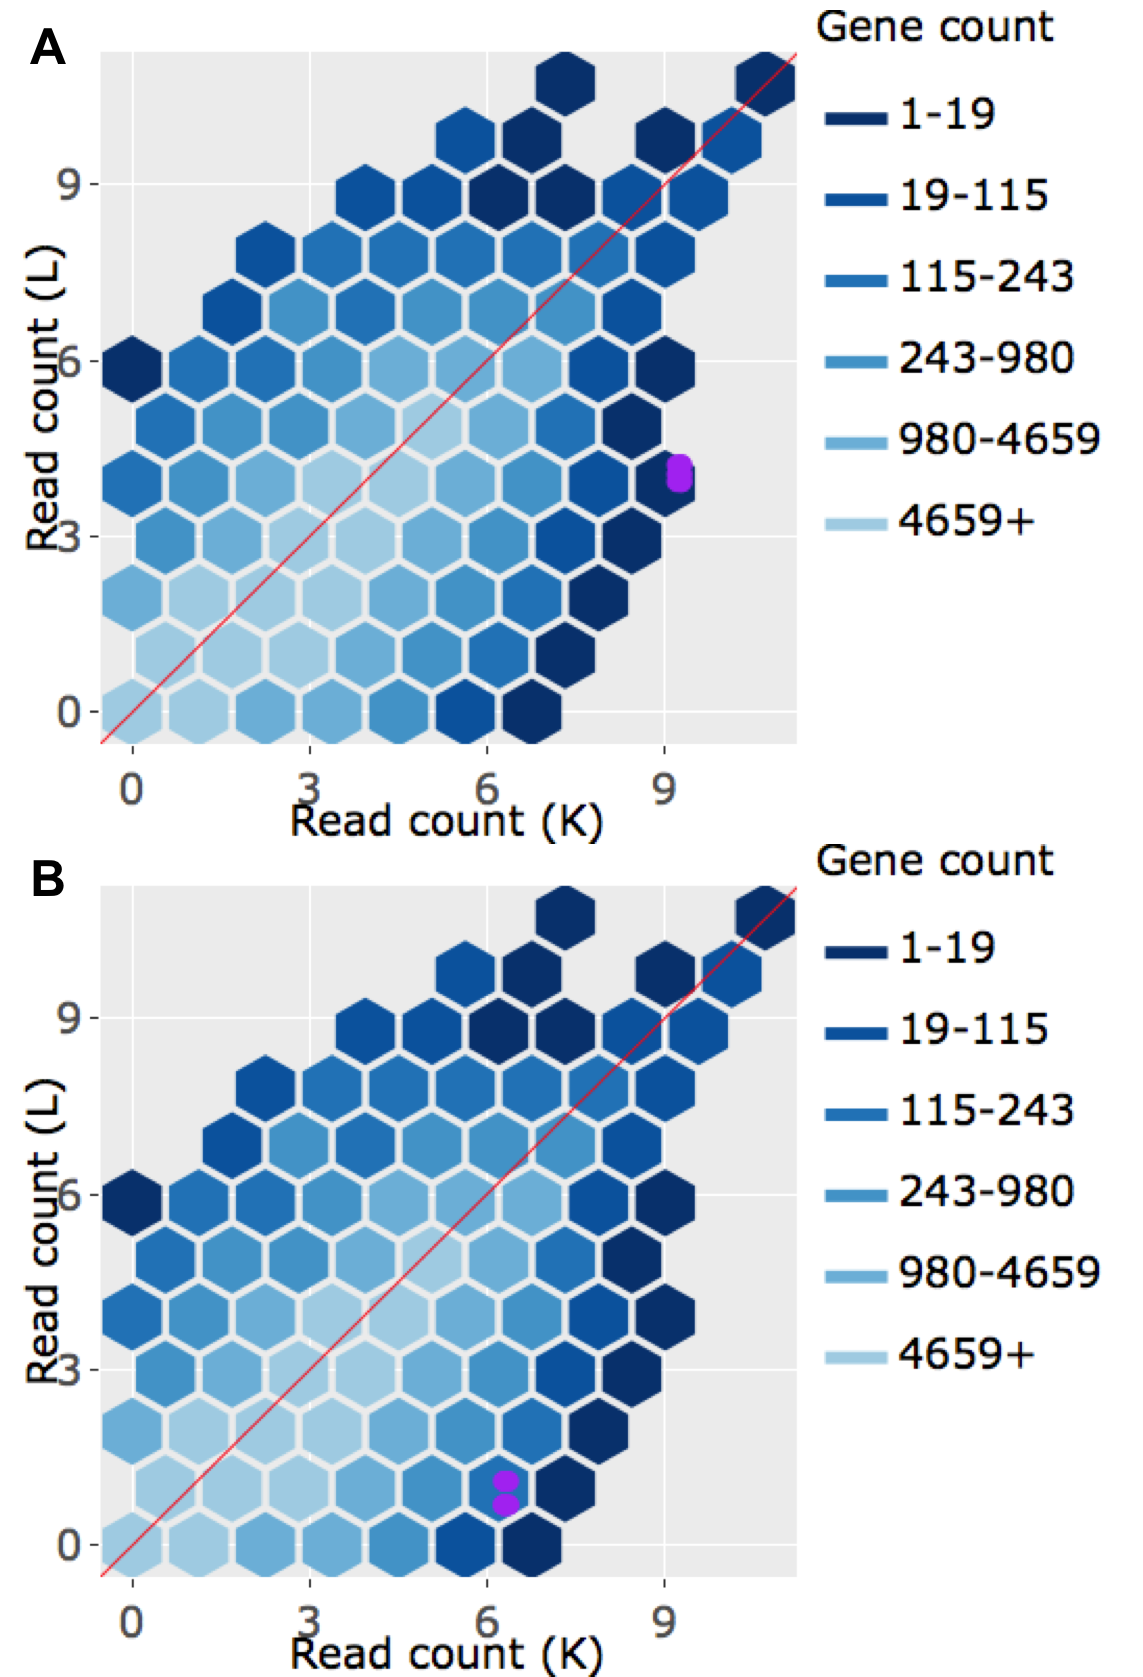
\includegraphics[width=0.7\columnwidth]{../Dashboards/exampleKeep.png}}
\caption{Example litre plots from the 1,136 genes that were in the first cluster (of Figure~\ref{KeepPCP}) of genes that remained kidney-specific DEGs even after TMM normalization. With these litre plots, we verify from an additional perspective that these genes demonstrate the expected patterns of DEGs.
\label{KeepLitre}}
\end{figure}

\null
\begin{figure}[t!]
\centerline{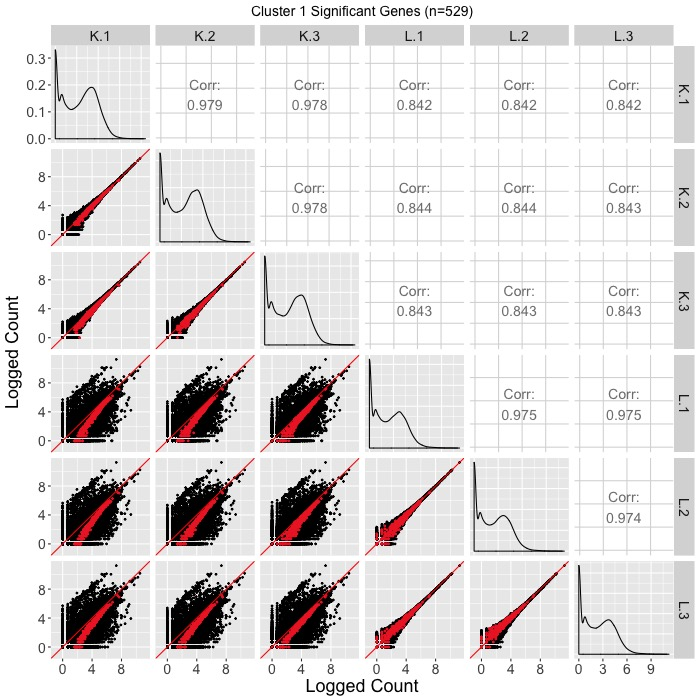
\includegraphics[width=1\columnwidth]{../Bioinformatics/Pictures/liverKidney/Clustering_data_FDR_001_TMMvRaw_Removed/K_L_Sig_SM_Removed_8_1.jpg}}
\caption{Scatterplot matrix of the 529 genes that were in the first cluster (of Figure~\ref{RemovePCP}) from genes that no longer remained as kidney-specific DEGs after TMM normalization. With this scatterplot matrix, we verify from an additional perspective that these genes do not demonstrate the expected patterns of DEGs too strongly (they do not deviate much from the \textit{x=y} line in the treatment scatterplots). This provides additional evidence that TMM normalization removing these genes from DEG status may be valid.
\label{RemovedSM}}
\end{figure}

\null
\begin{figure}[t!]
\centerline{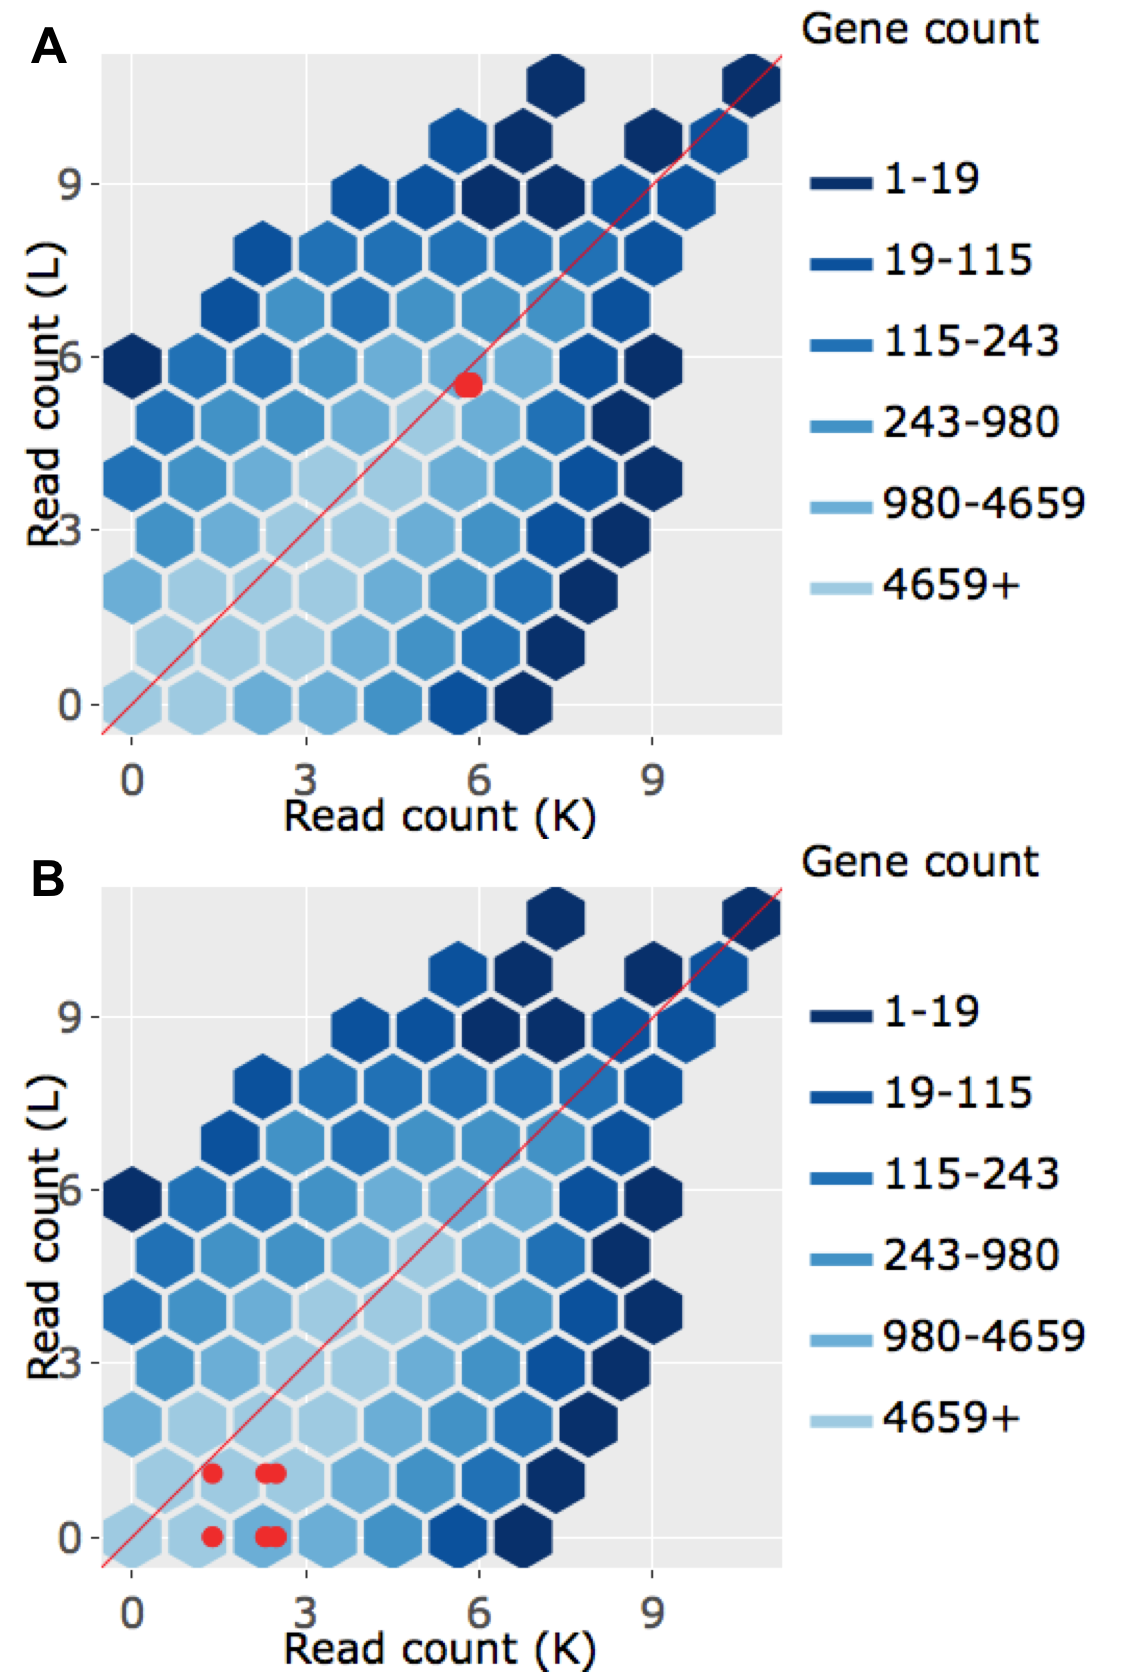
\includegraphics[width=0.7\columnwidth]{../Dashboards/exampleRemove.png}}
\caption{Example litre plots from the 529 genes that were in the first cluster (of Figure~\ref{RemovePCP}) of genes that no longer remained as kidney-specific DEGs after TMM normalization. With these litre plots, we verify from an additional perspective that these genes do not demonstrate the expected patterns of DEGs. This provides additional evidence that TMM normalization removing these genes from DEG status may be valid.
\label{RemovedLitre}}
\end{figure}


\null
\begin{figure}[t!]
\centerline{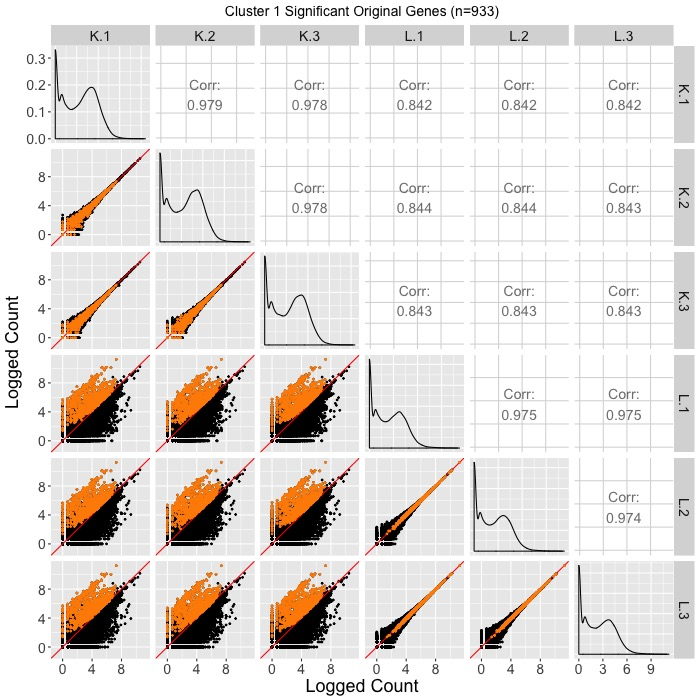
\includegraphics[width=1\columnwidth]{../Bioinformatics/Pictures/liverKidney/Clustering_data_FDR_001_TMMvRaw_Orig/K_L_Sig_SM_Orig_8_1.jpg}}
\caption{Scatterplot matrix of the 933 genes that were in the first cluster (of Figure~\ref{OrigPCP}) from genes that were initially designated as liver-specific DEGs after library scale normalization. With this scatterplot matrix, we verify from an additional perspective that these genes demonstrate the expected patterns of DEGs.
\label{OrigSM}}
\end{figure}

\null
\begin{figure}[t!]
\centerline{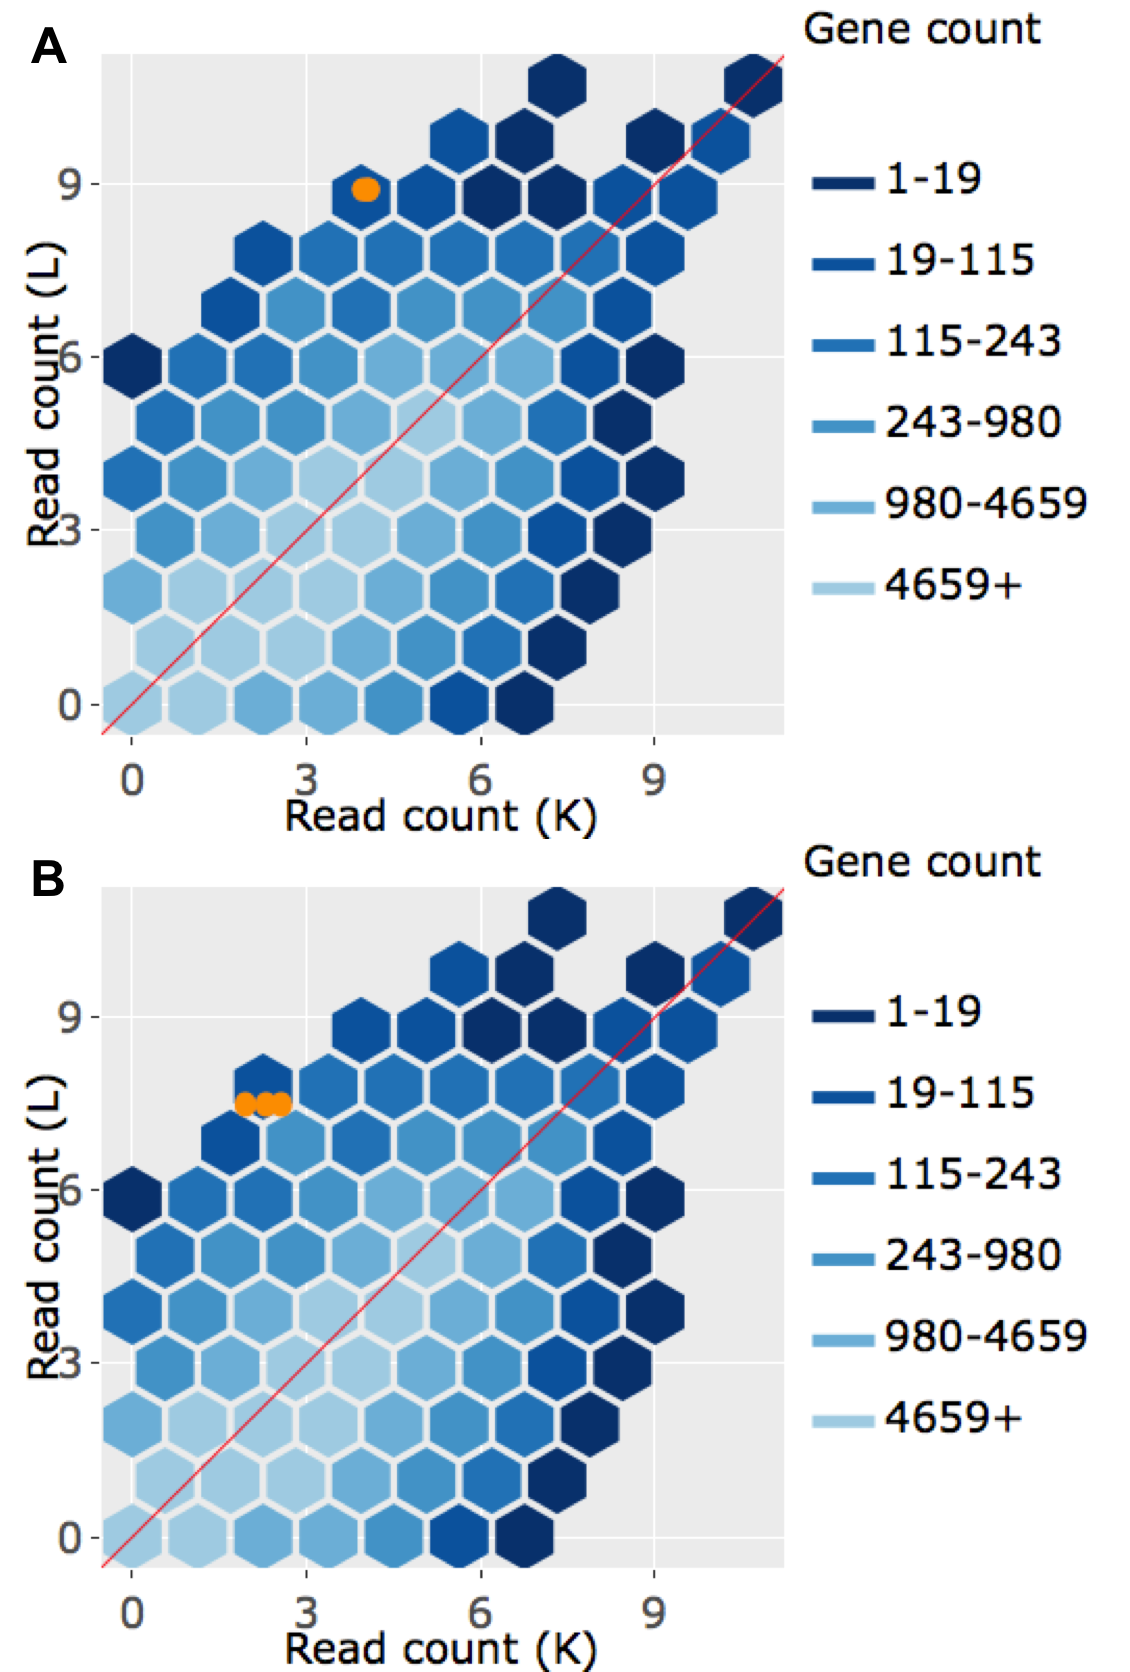
\includegraphics[width=0.7\columnwidth]{../Dashboards/exampleOrig.png}}
\caption{Example litre plots from the 933 genes that were in the first cluster (of Figure~\ref{OrigPCP}) from genes that were initially designated as liver-specific DEGs after library scale normalization. With these litre plots, we verify from an additional perspective that these genes demonstrate the expected patterns of DEGs.
\label{OrigLitre}}
\end{figure}


\null
\begin{figure}[t!]
\centerline{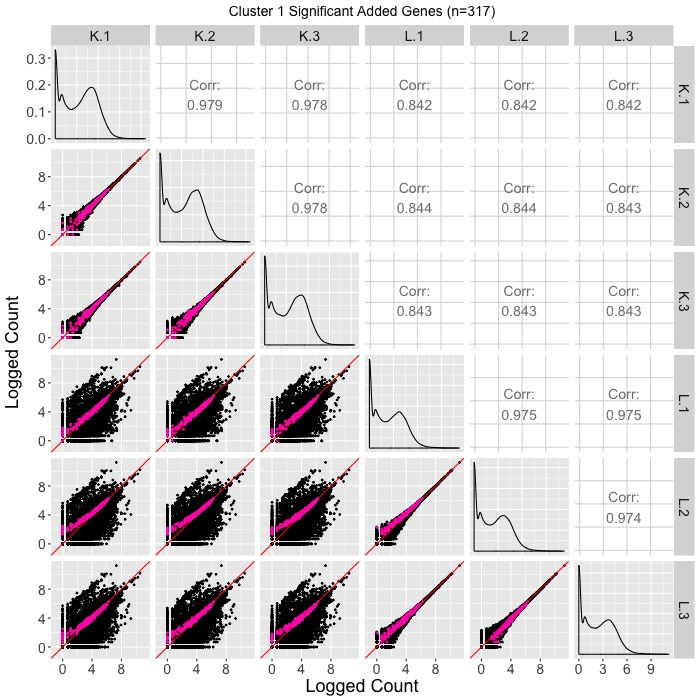
\includegraphics[width=1\columnwidth]{../Bioinformatics/Pictures/liverKidney/Clustering_data_FDR_001_TMMvRaw_Add/K_L_Sig_SM_Add_8_1.jpg}}
\caption{Scatterplot matrix of the 1,578 genes that were in the first cluster (of Figure~\ref{AddPCP}) from genes that were \textit{added} as liver-specific DEGs after TMM normalization. With this scatterplot matrix, we are \textbf{unable} to verify from an additional perspective that these genes demonstrate the expected patterns of DEGs. (Need to find an explanation for this).
\label{AddSM}}
\end{figure}

\null
\begin{figure}[t!]
\centerline{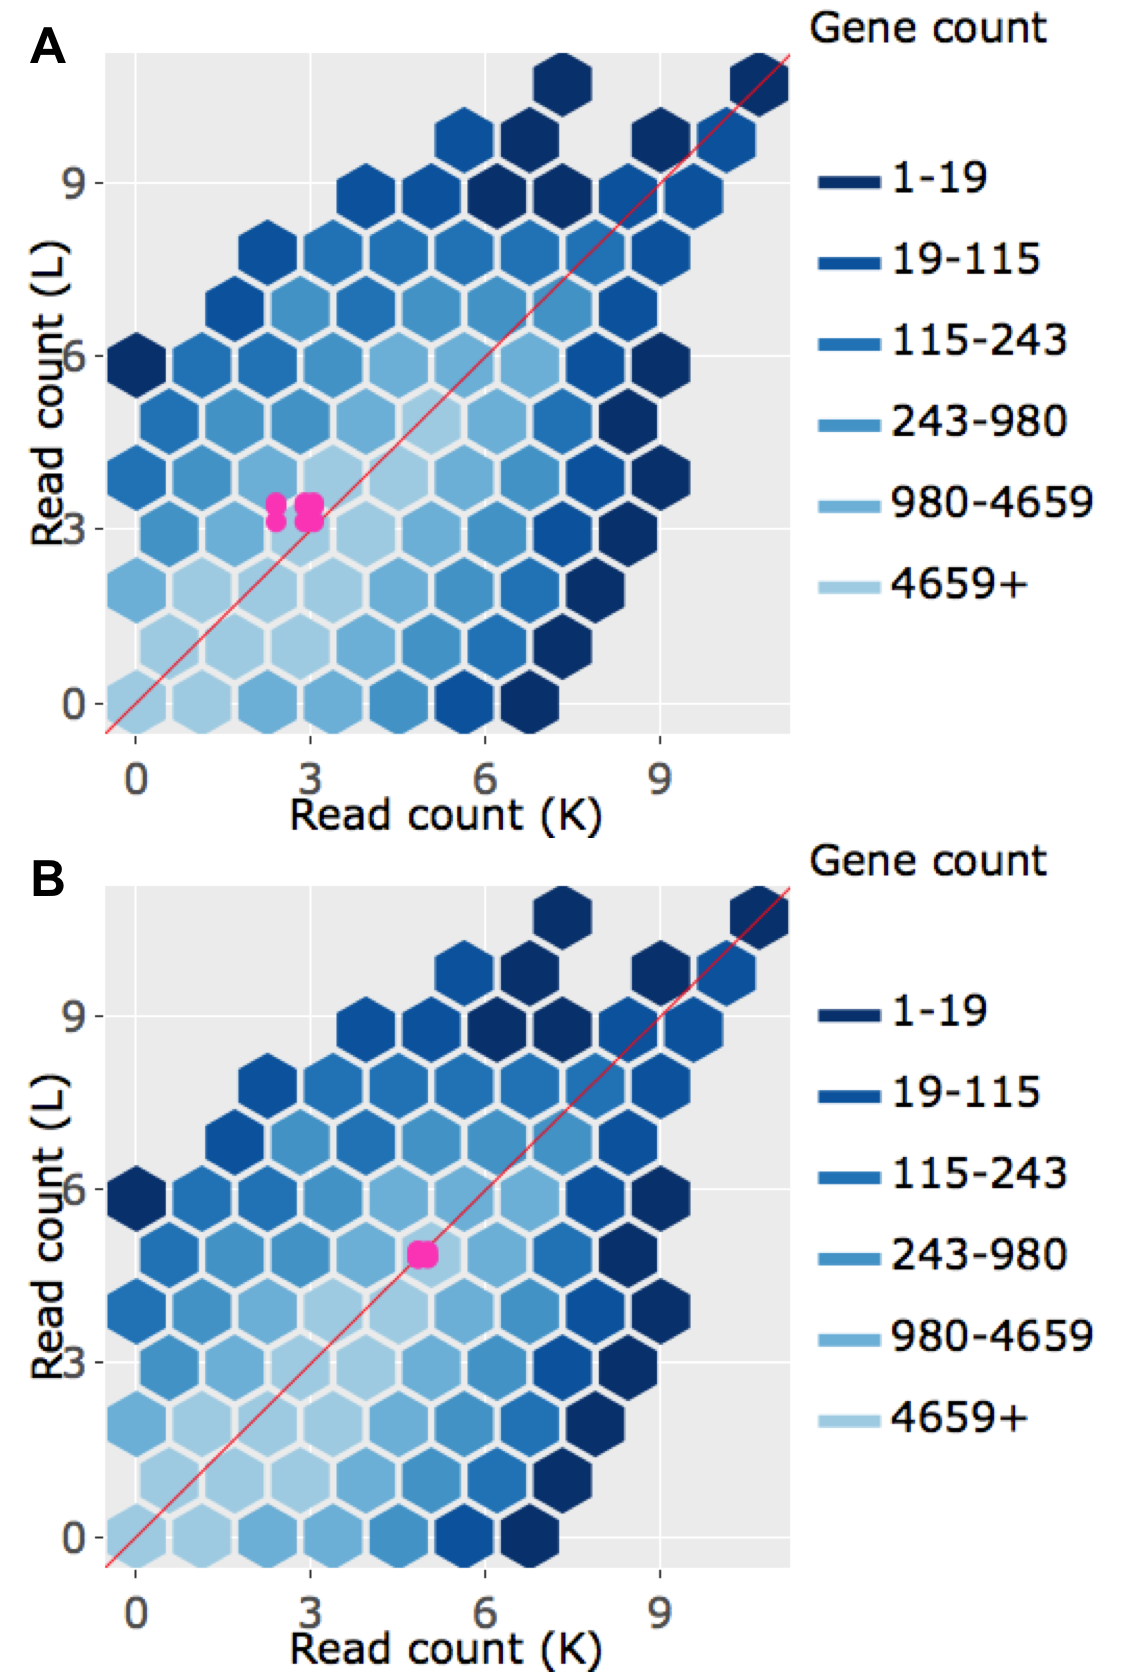
\includegraphics[width=0.7\columnwidth]{../Dashboards/exampleAdd.png}}
\caption{Example litre plots from the 1,578 genes that were in the first cluster (of Figure~\ref{AddPCP}) from genes that were \textit{added} as liver-specific DEGs after TMM normalization. With these litre plots, we are \textbf{unable} to verify from an additional perspective that these genes demonstrate the expected patterns of DEGs. (Need to find an explanation for this).
\label{AddLitre}}
\end{figure}

\end{document}